\documentclass{article}
\usepackage{color}
\usepackage{tikz}
\usepackage{pgfplotstable}
\usepackage{float}
\usepackage{tabularx}
\usepackage{amsmath}
\usepackage{amssymb}
\usepackage{listings}
\usepackage{enumitem}
\usepackage{syntax}
\usepackage{csquotes}
\usepackage{pgfplots}
%\usepackage[backend=biber]{biblatex}
%\addbibresource{references.bib}


\definecolor{dkgreen}{rgb}{0,0.6,0}
\definecolor{gray}{rgb}{0.5,0.5,0.5}
\definecolor{mauve}{rgb}{0.58,0,0.82}
\definecolor{variables}{RGB}{126,25,121}
\definecolor{symbolred}{RGB}{178,34,34}


\lstdefinelanguage{eprime}
{
	morekeywords={
		letting, be,
		indexed, by, of,
		given, 
		find,
		maximising, minimising,
		such, that,
		max, min,
		sum,
		forall, forAll, exists, alldifferent, table
	},
	morecomment=[l]{\$},
}

\lstset{
  language={eprime},
  frame=tb,
  alsoletter={\\}!.:+\=-<>{/}{..},
  emph = [1]{int, bool, matrix, domain},
  emphstyle = [1]{\color{variables}},
  emph = [2]{:, !=, ->, \=, +, -, ., .., *, \%, /\\, \\/, <, >, =},
  emphstyle = [2]{\color{symbolred}},  
  numbers=left,
  stepnumber=1,
  aboveskip=3mm,
  belowskip=3mm,
  showstringspaces=false,
  columns=flexible,
  basicstyle={\small\ttfamily},
  numberstyle=\color{gray},
  keywordstyle=\color{blue},
  commentstyle=\color{dkgreen},
  stringstyle=\color{mauve},
  breaklines=true,
  breakatwhitespace=true,
  tabsize=4,
  moredelim=**[is][\color{red}]{@}{@},  
}

\setlength{\grammarindent}{12em}

%\renewcommand{\lstlistingname}{Algorithm}
%\newcommand{\tablerow}[4]{ #1 & #2 & #3 & #4\\}
\newcommand{\n}[0]{\\[\baselineskip]}

%%%%
 % Macro for creating title page
 % #1 - Module code/name
 % #2 - Lecturer
%%%%
\newcommand{\maketitlepage}[2]{
\begin{titlepage}
	\centering
    \includegraphics[scale = 0.4]{01-standard-vertical-black.png}\\	% University Logo
	\textsc{\LARGE #1}\\[0.5 cm]				% Course Code
	\rule{\linewidth}{0.2 mm} \\[0.4 cm]
	{ \huge \bfseries \thetitle}
	\rule{\linewidth}{0.2 mm} \\[0.5 cm]
	\textsc{\large \thedate}\\[1.5 cm]
	
	\begin{minipage}{0.4\textwidth}
		\begin{flushleft} \large
			\emph{Lecturer:}\\
			#2
			\end{flushleft}
			\end{minipage}
			\begin{minipage}{0.4\textwidth}
            
			\begin{flushright} \large
			\emph{Submitted By:} \\
			\theauthor
		\end{flushright}
        
	\end{minipage}\\
	
\end{titlepage}
}

\title{The Bombastic Modelling Problem}
\author{140011146}

\makeatletter
\let\thetitle\@title
\let\theauthor\@author
\let\thedate\@date
\makeatother

\begin{document}

\maketitlepage{CS4402 Constraint Programming}{Ian Miguel}




\section{Introduction}
Bombastic is a Capcom video game which involves pushing dice on a grid into certain configurations. In this practical we take an abstraction of this game, modelling it in Essence Prime using the Savile Row tool and writing constraints to the problem. 
\n
The model and constraints are then run against a set of parameter files with different processing options in Savile Row to evaluate the performance of the model and explore the effects of heuristics and optimisations of the tool. 
\section{Design and Implementation}
An initial model was created to pass all tests from the given parameter files with little thought for efficiency. Afterwards, small changes were made to try and optimise the model and improve the time taken and reduce the number of solver nodes to search.
\subsection{Initial model}
\subsubsection{Initial and goal states}
There are three sets of state variables that need to be set up as the initial states: the avatar's position, the locations of the blocks and the cells of the grid. 

\begin{lstlisting}[caption={Constraints for setting initial state variables}, captionpos=b]
$ Avatar's initial position
avatarCurrentRow[0] = avatarInitRow,
avatarCurrentCol[0] = avatarInitCol,

$ Initial locations for blocks
forall block : int(1..numBlocks) .
    blocksCurrentRow[0,block] = blocksInitRow[block] /\
    blocksCurrentCol[0,block] = blocksInitCol[block],

$ Initial cells of grid
forall row : int(1..r) .
    forall col : int(1..c) .
        gridCurrent[0,row,col] = gridInit[row,col],
\end{lstlisting}
This sets all \texttt{current} decision variables for step 0 based on the given \texttt{init} parameter variables. All further constraints will be based on these \texttt{current} matrices and their values. Next is the constraint for the goal state.
\begin{lstlisting}[caption={Constraints for the goal state}, captionpos=b]
$ All blocks are in a goal
forall block : int(1..numBlocks) .
    exists goal : int(1..numBlocks) . 
        blocksCurrentRow[steps,block] = blocksGoalRow[goal] /\
		blocksCurrentCol[steps,block] = blocksGoalCol[goal],
\end{lstlisting}
Because it does not matter which blocks is pushed into which goal, we can say that for every block there must exist a goal it is in. This combined with the constraint that blocks cannot be in the same position means each block must be in a different goal.
\subsubsection{Invalid states}
Next are the constraints for invalid states of the game. This restricts the model to not have states such as having the avatar and a block be in the same position. 

\begin{lstlisting}[caption={Constraints to prevent invalid game states}, captionpos=b]
$ Avatar current row/col cannot be on dead cells
forall step : int(0..steps) .
    forall row : int(1..r) .
        forall col : int(1..c) .
	    	gridCurrent[step,row,col] = 0 
	    		-> avatarCurrentRow[step] != row \/ 
	    		   avatarCurrentCol[step] != col,


$ Blocks and avatar cannot share same cell
forall step : int(0..steps) .
    forall block : int(1..numBlocks) .
        avatarCurrentRow[step] != blocksCurrentRow[step,block] \/
		avatarCurrentCol[step] != blocksCurrentCol[step,block],

$ Block cannot be on dead cells
forall step : int(0..steps) .
    forall block : int(1..numBlocks) .
        forall row : int(1..r) .
	    forall col : int(1..c) .
	        gridCurrent[step,row,col] = 0 
	        	-> blocksCurrentRow[step,block] != row \/
				   blocksCurrentCol[step,block] != col,

$ Blocks cannot share same cell				       
forall step : int(0..steps) .
    forall checkBlock : int(1..numBlocks) .
        forall otherBlock : int(1..numBlocks) .
	    	checkBlock != otherBlock ->
	        	blocksCurrentRow[step, checkBlock] != blocksCurrentRow[step, otherBlock] \/
				blocksCurrentCol[step, checkBlock] != blocksCurrentCol[step, otherBlock],
\end{lstlisting}
All these constraints are quite similar and simply deal with not allowing the avatar or any blocks to share position or be in dead cells. An \vee is used instead of an \wedge because TODO


\subsubsection{Movement}
Now for movement. We need to ensure that if the \texttt{avatarCurrentRow} and \texttt{avatarCurrentCol} have different positions in different steps (i.e the avatar has moved its position), then \texttt{moveRol} and \texttt{moveCol} must be updated. Furthermore, the movement cannot be more than one step vertically or horizontally and not diagonally and there cannot be no movement every turn.

\begin{lstlisting}[caption={Updating \texttt{moveRow} and \texttt{moveCol}},captionpos=b]
$ Update moveRow/moveCol for avatar movement
forall step : int(1..steps) .
       moveRow[step] = avatarCurrentRow[step] - avatarCurrentRow[step-1] /\
       moveCol[step] = avatarCurrentCol[step] - avatarCurrentCol[step-1],

\end{lstlisting}
Updating \texttt{moveRow} and \texttt{moveCol} works as the game grid is indexed in order both row-wise and column-wise. To explain easily, we can rearrange the formula to be as follows:
\begin{lstlisting}
avatarCurrentRow[step] = moveRow[step] + avatarCurrentRow[step-1]
avatarCurrentCol[step] = moveCol[step] + avatarCurrentCol[step-1]
\end{lstlisting}
This intuitively says that the avatar's current position is its previous position plus the value of its movement. This works the same for a negative value of \texttt{moveRow}/\texttt{moveCol} as that is just moving in the other direction.
\begin{lstlisting}[caption={Prevent diagonal movement and force movement every turn}, captionpos=b]
$ Diagonal movement not allowed and must move each turn
forall step : int(1..steps) .
    | moveRow[step] | + | moveCol[step] | = 1,
\end{lstlisting}
The second constraint restricts both diagonal movement and forces the avatar to move every turn. This works because the absolute value of \texttt{moveRow} and \texttt{moveCol} is how much the avatar has moved by. To move diagonally, the sum of \texttt{moveRow} and \texttt{moveCol} must be at least 2, as one has to move at least one row \textit{and} column. Additionally, the avatar must move every turn with this constraint as the sum is equal to 1, so \texttt{moveRow} and \texttt{moveCol} cannot both be 0 on each turn. This also constrains the avatar to only move a distance of 1 each turn.
\n
Next, the blocks must be pushed by the avatar must be moved. To do this, two constraints were used.
\begin{lstlisting}[caption={Constraints for moving blocks}, captionpos=b]
$ If block has moved, avatar must have moved into block's previous location
forall step : int(1..steps) .
    forall block : int(1..numBlocks) .
        blocksCurrentRow[step-1,block] != blocksCurrentRow[step,block] \/
		blocksCurrentCol[step-1,block] != blocksCurrentCol[step,block] ->
	    	avatarCurrentRow[step] = blocksCurrentRow[step-1,block] /\
	    	avatarCurrentCol[step] = blocksCurrentCol[step-1,block],

$ If avatar moved into block, block move same direction
forall step : int(1..steps) .
    forall block : int(1..numBlocks) .
        avatarCurrentRow[step] = blocksCurrentRow[step-1,block] /\
		avatarCurrentCol[step] = blocksCurrentCol[step-1,block] ->
	    	blocksCurrentRow[step,block] = blocksCurrentRow[step-1,block] + moveRow[step] /\
	    	blocksCurrentCol[step,block] = blocksCurrentCol[step-1,block] + moveCol[step],
\end{lstlisting}
The first checks if a block has moved on the next step. If the block has moved, then the avatar must have moved into the block's old position as that is the only way blocks can move. However, just this constraint is not enough as it doesn't say anything about how to move the block. The second constraint moves the block by adding \texttt{moveRow} and \texttt{moveCol} to \texttt{blocksCurrentRow} and \texttt{blocksCurrentCol} respectively. This works as \texttt{moveRow} and \texttt{moveCol} directly represent the direction of the avatar's movement and blocks must be pushed in the same direction. We do not have to worry about pushing blocks into dead cells as previous constraints do not allow that to happen. 


\subsubsection{Grid and ice}
Finally, we have to make sure than none of the grid changes unless it is ice and it was stepped on.

\begin{lstlisting}[caption={Constraints for grid cells}, captionpos=b]
$ Grid 0 and 2s always stay the same
forall step : int(1..steps) .
    forall row : int(1..r) .
        forall col : int(1..c) .
	    	gridCurrent[step-1,row,col] != 1 ->
	        	gridCurrent[step,row,col] = gridCurrent[step-1,row,col],

$ Ice becomes dead cell
forall step : int(1..steps) .
    forall row : int(1..r) .
        forall col : int(1..c) .
	    	avatarCurrentRow[step-1] = row /\
	    	avatarCurrentCol[step-1] = col /\
	    	gridCurrent[step-1,row,col] = 1 ->
	        	gridCurrent[step,row,col] = 0,
\end{lstlisting}
The first constraint here ensures 0s and 2s never change, however this doesn't take into account the 1s that need to stay the same as long as the avatar has not stepped on them yet. 
\begin{lstlisting}[caption={Additional constraint to prevent ice cells from changing}, captionpos=b]
$Ice not stepped on doesn't change
forall step : int(1..steps) .
    forall row : int(1..r) .
        forall col : int(1..c) .
	    	gridCurrent[step-1,row,col] = 1 /\
	    	(avatarCurrentRow[step-1] != row \/ 
	     	avatarCurrentCol[step-1] != col) ->
	        	gridCurrent[step,row,col] = 1

\end{lstlisting}
For this constraint, in addition to the grid of the previous step having to be an ice cell (\texttt{gridCurrent[step-1,row,col] = 1}), the avatar must also not have stepped on the cell in the previous turn. Only then should the ice cells stay the same.
\subsection{Model improvements}
After some testing and initial results, improvements to the original model were made that substantially reduced the number of solver nodes. 
\subsubsection{Direct row/col}
In a few cases, the constraints in the initial model had to loop through all steps, rows and columns, for example to check the avatar is not on a dead cell. This could be simplified to directly use the avatar's current row and column as an index rather than check every combination of step, row and col.
\begin{lstlisting}[caption={Example of optimising number of constraints by directly indexing with \texttt{avatarCurrentRow} and \texttt{avatarCurrentCol}.}, captionpos=b]
$ Avatar current row/col cannot be on dead cells
forall step : int(0..steps) .
    forall row : int(1..r) .
        forall col : int(1..c) .
	    	gridCurrent[step,row,col] = 0 -> 
	    		avatarCurrentRow[step] != row \/ 
	    		avatarCurrentCol[step] != col,

$ Optimisation
forall step : int (0..steps) .
    gridCurrent[step, avatarCurrentRow[step], avatarCurrentCol[step]] != 0,
\end{lstlisting}
Other constraints of this pattern, such as checking a block on a dead cell were all changed the same way.

\section{Experimentation}
The constraint models were tested on the given parameter files and the results of the \texttt{.info} files taken. The results are then displayed and analysed to test differences in optimisation and heuristic options in Savile Row. Finally, new instances were created and tested TODO


\subsection{Methodology}

For the experiments with optimisation and heuristic options in Savile Row, both the initial model and improved model were used. This lets us see if any options can improve the efficiency in which the models find solutions without manually refining the constraints. 
\n
The time taken by the solver is not the best metric to look at, as it is not the same on every run and dependent on the load and speed of the computer running the experiment. The number of solver nodes will also be used as a metric of how well the models perform since this number will always stay the same for the same model and problem instance. 

\begin{figure}[H]
\centering
\begin{minipage}{0.4\textwidth}
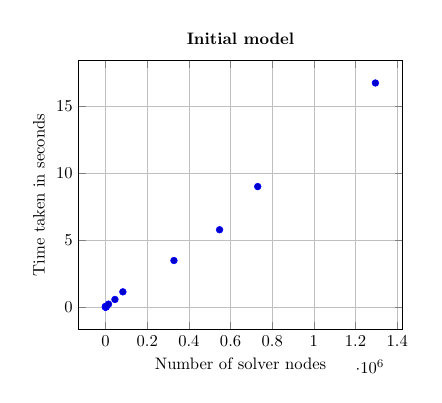
\begin{tikzpicture}[scale=0.6]
\begin{axis}[
	title={\textbf{Initial model}},
	ylabel={Time taken in seconds},
	xlabel={Number of solver nodes},
	ymajorgrids=true,
	xmajorgrids=true,
	legend pos=north west,
	]
	
\addplot+[only marks, mark=*] table {
1 0.033224             
0 0.000586             
1 0.030841             
0 0.000814             
19 0.03524             
0 0.001459             
18 0.038105            
267 0.006645           
615 0.044015           
7052 0.099708          
14036 0.225809         
44769 0.574981         
82920 1.1448           
328143 3.48632         
730259 9.01066         
547184 5.78452         
1295335 16.7512
};
\label{plot:initial-model}
\end{axis}
\end{tikzpicture}
\end{minipage}
%
\begin{minipage}{0.4\textwidth}
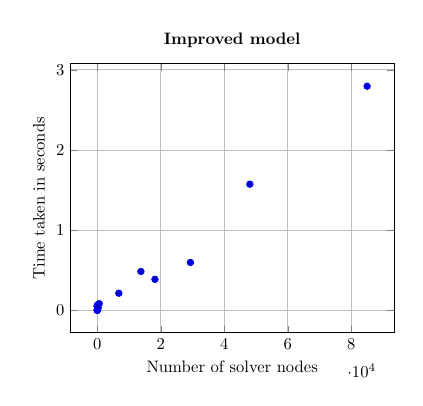
\begin{tikzpicture}[scale=0.6]
\begin{axis}[
	title={\textbf{Improved model}},
	ylabel={Time taken in seconds},
	xlabel={Number of solver nodes},
	ymajorgrids=true,
	xmajorgrids=true,
	legend pos=north west,
	]
	
\addplot+[only marks, mark=*] table {
1 0.047307                                     
0 0.0                                          
1 0.047608                                     
0 0.000834                                     
19 0.065945                                    
0 0.001938                                     
1 0.049589                                     
267 0.02942                                    
615 0.083765                                   
6786 0.213979                                  
13737 0.484895                                 
0 0.007957                                     
1 0.047291                                     
18169 0.387194                                 
48055 1.57321                                  
29331 0.597242                                 
85000 2.79481 
};

\label{plot:initial-model}
\end{axis}
\end{tikzpicture}
\end{minipage}
\caption{Number of solver nodes plotted against time for both initial and improved models. We can see a strong linear relationship between the time taken and number of solver nodes. This shows both are equivalent metrics for measuring the performance of our model.}
\label{fig:solver-time}
\end{figure}
\noindent
To run the experiments, a simple python script was written to run Savile Row automatically with various options and the results gathered. 
\subsection{Results}

\begin{figure}[H]
\centering
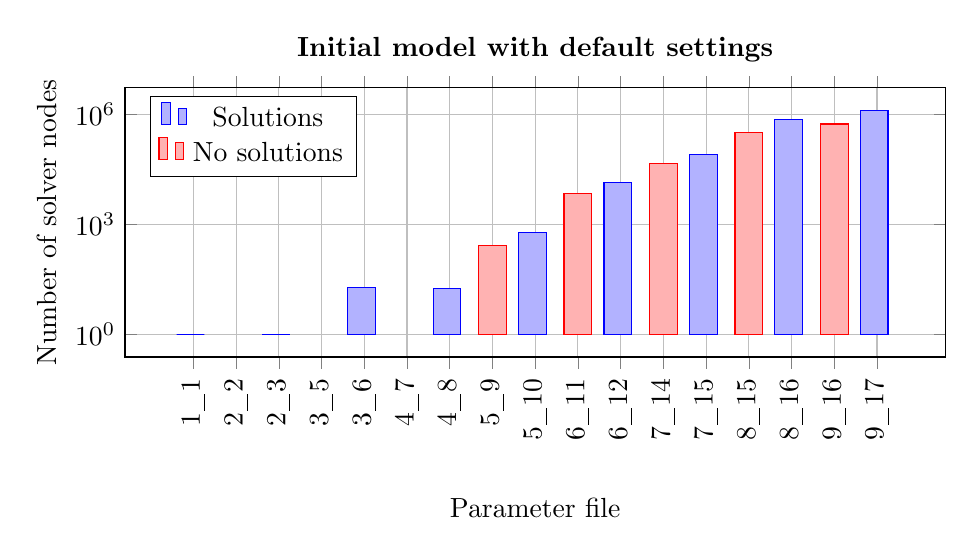
\begin{tikzpicture}
\begin{axis}[
	title={\textbf{Initial model with default settings}},
	ybar,
	bar width=1em,
	width=12cm,
	height=5cm,
	ylabel={Number of solver nodes},
	ymode=log,
	xlabel={Parameter file},
	x label style={yshift=-0.5cm},
	xtick={1,2,3,4,5,6,7,8,9,10,11,12,13,14,15,16,17},
	xticklabels={1_1, 2_2, 2_3, 3_5, 3_6, 4_7, 4_8, 5_9, 5_10, 6_11, 6_12, 7_14, 7_15, 8_15, 8_16, 9_16, 9_17},
	x tick label style={rotate=90, anchor=east},
	ymajorgrids=true,
	xmajorgrids=true,
	legend pos=north west,
]

\addplot+[
xshift=0.5em, 
legend image post style={xshift=-0.5em}
] 
coordinates { (1,1) (3,1) (5,19) (7,18) (9,615) (11,14036) (13,82920) (15,730243) (17,1295303) };
\label{plot:solution-node}
\addlegendentry{Solutions}

\addplot+[
xshift=-0.6em,
legend image post style={xshift=0.5em}
] 
coordinates { (2,0) (4,0) (6,0) (8,267) (10,7052) (12,44769) (14,328143) (16,547184) };
\label{plot:nosolution-node}
\addlegendentry{No solutions}

\end{axis}
\end{tikzpicture}
\n
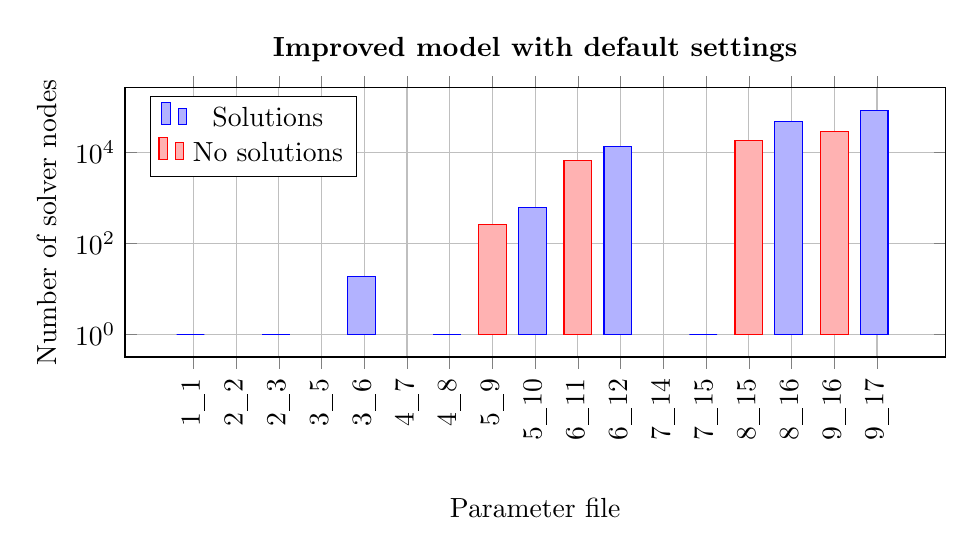
\begin{tikzpicture}
\begin{axis}[
	title={\textbf{Improved model with default settings}},
	ybar,
	bar width=1em,
	width=12cm,
	height=5cm,
	ylabel={Number of solver nodes},
	ymode=log,
	xlabel={Parameter file},
	x label style={yshift=-0.5cm},
	xtick={1,2,3,4,5,6,7,8,9,10,11,12,13,14,15,16,17},
	xticklabels={1_1, 2_2, 2_3, 3_5, 3_6, 4_7, 4_8, 5_9, 5_10, 6_11, 6_12, 7_14, 7_15, 8_15, 8_16, 9_16, 9_17},
	x tick label style={rotate=90, anchor=east},
	ymajorgrids=true,
	xmajorgrids=true,
	legend pos=north west,
]

\addplot+[
xshift=0.5em, 
legend image post style={xshift=-0.5em}
] 
coordinates { (1,1) (3,1) (5,19) (7,1) (9,615) (11,13737) (13,1) (15,48055) (17,85000) };
\label{plot:solution-node}
\addlegendentry{Solutions}

\addplot+[
xshift=-0.6em,
legend image post style={xshift=0.5em}
] 
coordinates { (2,0) (4,0) (6,0) (8,267) (10,6786) (12,0) (14,18169) (16,29331) };
\label{plot:nosolution-node}
\addlegendentry{No solutions}

\end{axis}
\end{tikzpicture}
\caption{Time taken and number of solver nodes for all given parameters}
\end{figure}



\begin{figure}[H]

\end{figure}

\subsubsection{Optimisations}

\begin{figure}[H]
\centering
\begin{minipage}{0.45\textwidth}
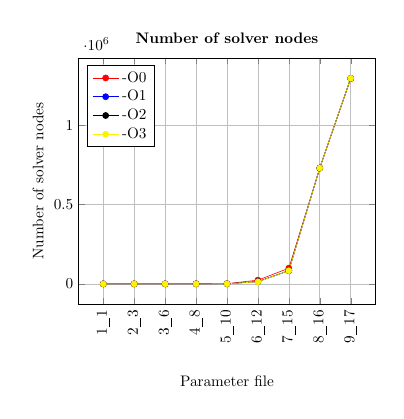
\begin{tikzpicture}[scale=0.55]
\begin{axis}[
	title={\textbf{Number of solver nodes}},
	ylabel={Number of solver nodes},
	%ymode=log,
	xlabel={Parameter file},
	x label style={yshift=-0.5cm},
	xtick={1,3,5,7,9,11,13,15,17},
	xticklabels={1_1, 2_3, 3_6, 4_8, 5_10, 6_12, 7_15, 8_16, 9_17},
	x tick label style={rotate=90, anchor=east},
	ymajorgrids=true,
	xmajorgrids=true,
	legend pos=north west,
	cycle list name=color list,
	]

\addplot+[mark=*] coordinates {
(1,1) (3,1) (5,21) (7,266) (9,1322) (11,23368) (13,98601) (15,729172) (17,1293411) };
\label{plot:solution-node-o0}
\addlegendentry{-O0}

\addplot+[mark=*] coordinates {
(1,1) (3,1) (5,19) (7,18) (9,615) (11,14036) (13,82920) (15,730259) (17,1295335)};
\label{plot:solution-node-o1}
\addlegendentry{-O1}

\addplot+[mark=*] coordinates {
(1,1) (3,1) (5,19) (7,18) (9,615) (11,14036) (13,82920) (15,730259) (17,1295335)};
\label{plot:solution-node-o2}
\addlegendentry{-O2}

\addplot+[mark=*] coordinates {
(1,1) (3,1) (5,19) (7,18) (9,615) (11,12838) (13,82920) (15,730259) (17,1295335)};
\label{plot:solution-node-o3}
\addlegendentry{-O3}

\end{axis}

\end{tikzpicture}
\end{minipage}
%
\begin{minipage}{0.45\textwidth}
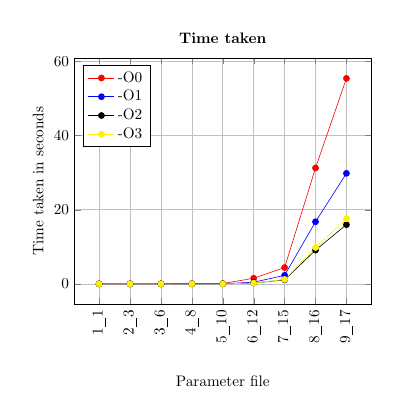
\begin{tikzpicture}[scale=0.55]
\begin{axis}[
	title={\textbf{Time taken}},
	ylabel={Time taken in seconds},
	%ymode=log,
	xlabel={Parameter file},
	x label style={yshift=-0.5cm},
	xtick={1,3,5,7,9,11,13,15,17},
	xticklabels={1_1, 2_3, 3_6, 4_8, 5_10, 6_12, 7_15, 8_16, 9_17},
	x tick label style={rotate=90, anchor=east},
	ymajorgrids=true,
	xmajorgrids=true,
	legend pos=north west,
	cycle list name=color list,
	]

\addplot+[mark=*] coordinates {
(1,0.034987) (3,0.037164) (5,0.049465) (7,0.066688) (9,0.123698) (11,1.54227) (13,4.42801) (15,31.2728) (17,55.4183)
};
\label{plot:nosolution-time-o0}
\addlegendentry{-O0}

\addplot+[mark=*] coordinates {
(1,0.03391) (3,0.033884) (5,0.041397) (7,0.055702) (9,0.066537) (11,0.476045) (13,2.33189) (15,16.768) (17,29.8262)};
\label{plot:nosolution-time-o1}
\addlegendentry{-O1}

\addplot+[mark=*] coordinates {
(1,0.034406) (3,0.033279) (5,0.037437) (7,0.037128) (9,0.045367) (11,0.239904) (13,1.1221) (15,9.12738) (17,15.9849)};
\label{plot:nosolution-time-o2}
\addlegendentry{-O2}

\addplot+[mark=*] coordinates {
(1,0.034467) (3,0.037342) (5,0.036098) (7,0.037964) (9,0.045614) (11,0.228288) (13,1.22769) (15,9.84382) (17,17.5615)};
\label{plot:nosolution-time-o3}
\addlegendentry{-O3}

\end{axis}
\end{tikzpicture}
\end{minipage}
\caption{Comparing the effect of optimisation flags on the number of nodes and time taken on the initial model for parameter files with solutions. See appendix TODO for full results.}
\end{figure}
\noindent
An interesting result from using different optimisation flags in Savile Row is the effect it has on the performance of the model. Although it was shown earlier that the number of solver nodes and the time taken by the solver are equivalent for measuring the performance of the model, the optimisation flags have a much greater effect on the time taken compared to the number of nodes the solver has to search. With optimisations, the number of solver nodes only decreased by a small fraction. For many parameter files, this number did not change between the three levels of optimisation. However for the time taken by the solver, the time almost halved for most parameter files when comparing \texttt{-O0} and \texttt{-O1}. The time again decreased significantly for \texttt{-O2}, though there is little difference between \texttt{-O2} and \texttt{-O3}.
\begin{figure}[H]
\centering
\begin{minipage}{0.45\textwidth}
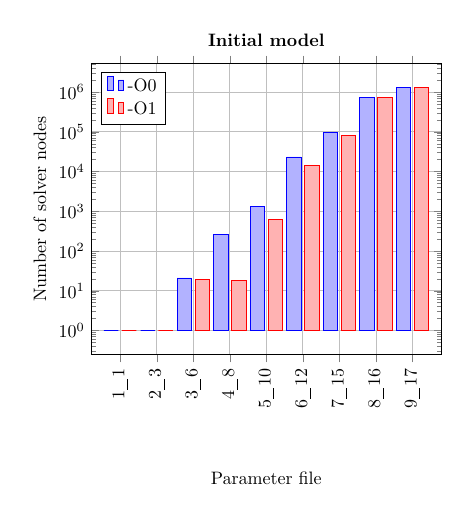
\begin{tikzpicture}[scale=0.65]
\begin{axis}[
	title={\textbf{Initial model}},
	ybar,
	bar width=0.8em,
	ylabel={Number of solver nodes},
	ymode=log,
	xlabel={Parameter file},
	x label style={yshift=-1cm},
	xtick={1,3,5,7,9,11,13,15,17},
	xticklabels={1_1, 2_3, 3_6, 4_8, 5_10, 6_12, 7_15, 8_16, 9_17},
	x tick label style={rotate=90, anchor=east},
	ymajorgrids=true,
	xmajorgrids=true,
	legend pos=north west,
	]

\addplot coordinates {
(1,1) (3,1) (5,21) (7,266) (9,1322) (11,23368) (13,98601) (15,729172) (17,1293411)
};
\label{plot:nosolution-time-o0}
\addlegendentry{-O0}

\addplot coordinates {
(1,1) (3,1) (5,19) (7,18) (9,615) (11,14036) (13,82920) (15,730259) (17,1295335)};
\label{plot:nosolution-time-o1}
\addlegendentry{-O1}
\end{axis}
\end{tikzpicture}
\end{minipage}
%
\begin{minipage}{0.45\textwidth}
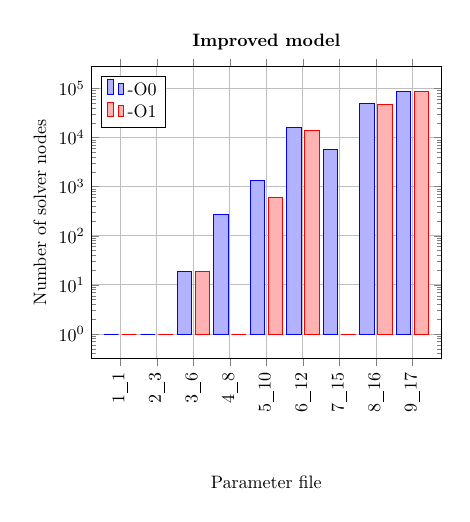
\begin{tikzpicture}[scale=0.65]
\begin{axis}[
	title={\textbf{Improved model}},
	ybar,
	bar width=0.8em,
	ylabel={Number of solver nodes},
	ymode=log,
	xlabel={Parameter file},
	x label style={yshift=-1cm},
	xtick={1,3,5,7,9,11,13,15,17},
	xticklabels={1_1, 2_3, 3_6, 4_8, 5_10, 6_12, 7_15, 8_16, 9_17},
	x tick label style={rotate=90, anchor=east},
	ymajorgrids=true,
	xmajorgrids=true,
	legend pos=north west,
	]

\addplot coordinates {
(1,1) (3,1) (5,19) (7,266) (9,1313) (11,16198) (13,5755) (15,49723) (17,88077)
};
\label{plot:nosolution-time-o0}
\addlegendentry{-O0}

\addplot coordinates {
(1,1) (3,1) (5,19) (7,1) (9,615) (11,13737) (13,1) (15,48055) (17,85000)};
\label{plot:nosolution-time-o1}
\addlegendentry{-O1}
\end{axis}
\end{tikzpicture}
\end{minipage}
\caption{Effect of optimisation flags on number of solver nodes for parameter files with solutions.}
\label{fig:optimisation-nodes}
\end{figure}
\noindent
This shows that parts of the optimisation is optimising Savile Row like a program, similar to how optimisation flags work in compilers like \texttt{gcc} rather than optimising it as a constraint solver. These optimisations would work well for most general programs, speeding up the run time but does little to improve our model from a constraint programming point of view. That is not to say the optimisations have no effect at all on the constraints. Figure \ref{fig:optimisation-nodes} shows that for some parameter files, the optimisation does well enough to eliminate many solver nodes. From the difference shown between the initial model and improved model, it can be seen that the optimisations have a stronger effect on the better model. 


\subsubsection{Heuristics}
Another option to look at is the heuristics that Essence Prime provides. As these are heuristics that must be specified in the model (in \texttt{Bombastic.eprime}), they should only affect the number of solver nodes and not the time taken by Savile Row. 
\begin{figure}[H]
\centering
\begin{minipage}{0.4\textwidth}
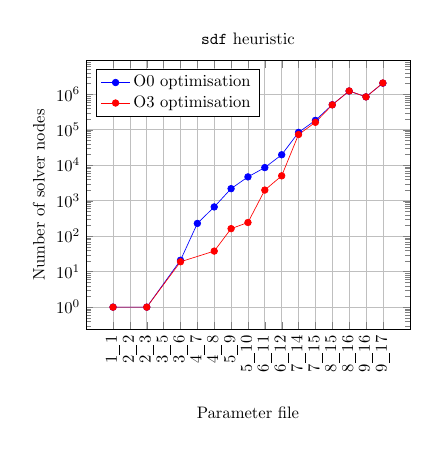
\begin{tikzpicture}[scale=0.6]
\begin{axis}[
	title={\texttt{sdf} heuristic},
	ylabel={Number of solver nodes},
	ymode=log,
	xlabel={Parameter file},
	x label style={yshift=-0.5cm},
	xtick={1,2,3,4,5,6,7,8,9,10,11,12,13,14,15,16,17},
	xticklabels={1_1, 2_2, 2_3, 3_5, 3_6, 4_7, 4_8, 5_9, 5_10, 6_11, 6_12, 7_14, 7_15, 8_15, 8_16, 9_16, 9_17},
	x tick label style={rotate=90, anchor=east},
	ymajorgrids=true,
	xmajorgrids=true,
	legend pos=north west,
	]

\addplot[color=blue, mark=*,] coordinates { (1,1) (2,0) (3,1) (4,0) (5,21) (6,229) (7,668) (8,2184) (9,4688) (10,8579) (11,19720) (12,84300) (13,183603) (14,507126) (15,1230659) (16,844406) (17,2055840)};
\label{plot:sdf-o0}
\addlegendentry{O0 optimisation}

\addplot[color=red, mark=*,] coordinates { (1,1) (2,0) (3,1) (4,0) (5,19) (6,0) (7,38) (8,163) (9,243) (10,1994) (11,5021) (12,73418) (13,162024) (14,502477) (15,1239351) (16,841628) (17,2077990)};
\label{plot:sdf-o3}
\addlegendentry{O3 optimisation}

\end{axis}
\end{tikzpicture}
\end{minipage}
%
\begin{minipage}{0.4\textwidth}
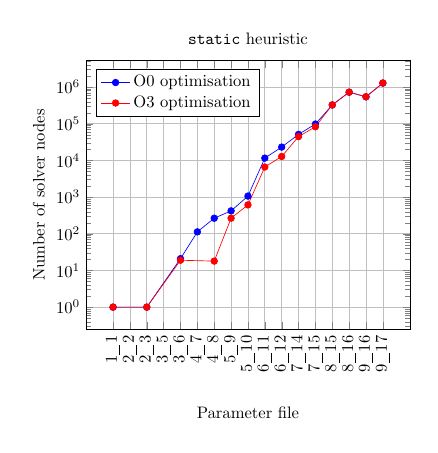
\begin{tikzpicture}[scale=0.6]
\begin{axis}[
	title={\texttt{static} heuristic},
	ylabel={Number of solver nodes},
	ymode=log,
	xlabel={Parameter file},
	x label style={yshift=-0.5cm},
	xtick={1,2,3,4,5,6,7,8,9,10,11,12,13,14,15,16,17},
	xticklabels={1_1, 2_2, 2_3, 3_5, 3_6, 4_7, 4_8, 5_9, 5_10, 6_11, 6_12, 7_14, 7_15, 8_15, 8_16, 9_16, 9_17},
	x tick label style={rotate=90, anchor=east},
	ymajorgrids=true,
	xmajorgrids=true,
	legend pos=north west,
]

\addplot[color=blue, mark=*,] coordinates { (1,1) (2,0) (3,1) (4,0) (5,21) (6,113) (7,266) (8,422) (9,1068) (10,11586) (11,23143) (12,51454) (13,98558) (14,324862) (15,725870) (16,542821) (17,1287730) };
\label{plot:static-o0}
\addlegendentry{O0 optimisation}

\addplot[color=red, mark=*,] coordinates { (1,1) (2,0) (3,1) (4,0) (5,19) (6,0) (7,18) (8,267) (9,615) (10,6622) (11,12838) (12,44769) (13,82920) (14,328133) (15,730243) (16,547164) (17,1295303) };
\label{plot:static-o3}
\addlegendentry{O3 optimisation}

\end{axis}
\end{tikzpicture}
\end{minipage}
\n
\begin{minipage}{0.4\textwidth}
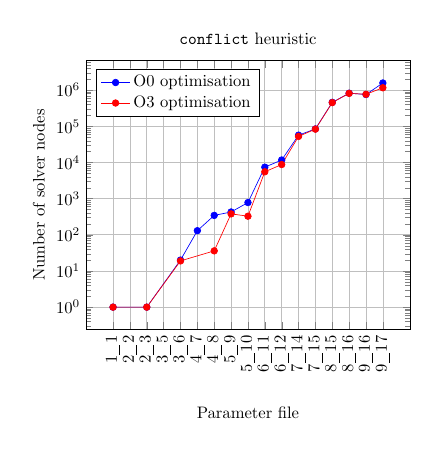
\begin{tikzpicture}[scale=0.6]
\begin{axis}[
	title={\texttt{conflict} heuristic},
	ylabel={Number of solver nodes},
	ymode=log,
	xlabel={Parameter file},
	x label style={yshift=-0.5cm},
	xtick={1,2,3,4,5,6,7,8,9,10,11,12,13,14,15,16,17},
	xticklabels={1_1, 2_2, 2_3, 3_5, 3_6, 4_7, 4_8, 5_9, 5_10, 6_11, 6_12, 7_14, 7_15, 8_15, 8_16, 9_16, 9_17},
	x tick label style={rotate=90, anchor=east},
	ymajorgrids=true,
	xmajorgrids=true,
	legend pos=north west,
]

\addplot[color=blue, mark=*,] coordinates { (1,1) (2,0) (3,1) (4,0) (5,20) (6,130) (7,344) (8,427) (9,780) (10,7417) (11,11686) (12,56819) (13,84540) (14,459939) (15,821932) (16,756356) (17,1575077)};
\label{plot:srf-o0}
\addlegendentry{O0 optimisation}

\addplot[color=red, mark=*,] coordinates { (1,1) (2,0) (3,1) (4,0) (5,19) (6,0) (7,36) (8,379) (9,327) (10,5520) (11,8760) (12,52563) (13,83408) (14,452072) (15,814969) (16,767724) (17,1163210) };
\label{plot:srf-o3}
\addlegendentry{O3 optimisation}

\end{axis}
\end{tikzpicture}
\end{minipage}
%
\begin{minipage}{0.4\textwidth}
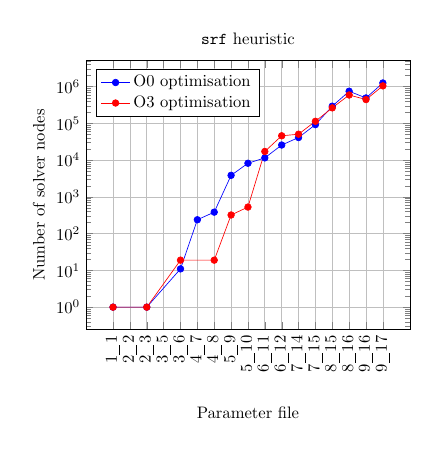
\begin{tikzpicture}[scale=0.6]
\begin{axis}[
	title={\texttt{srf} heuristic},
	ylabel={Number of solver nodes},
	ymode=log,
	xlabel={Parameter file},
	x label style={yshift=-0.5cm},
	xtick={1,2,3,4,5,6,7,8,9,10,11,12,13,14,15,16,17},
	xticklabels={1_1, 2_2, 2_3, 3_5, 3_6, 4_7, 4_8, 5_9, 5_10, 6_11, 6_12, 7_14, 7_15, 8_15, 8_16, 9_16, 9_17},
	x tick label style={rotate=90, anchor=east},
	ymajorgrids=true,
	xmajorgrids=true,
	legend pos=north west,
]

\addplot[color=blue, mark=*,] coordinates { (1,1) (2,0) (3,1) (4,0) (5,11) (6,239) (7,385) (8,3864) (9,8240) (10,11543) (11,25800) (12,41280) (13,92541) (14,294335) (15,750655) (16,492809) (17,1259049) };
\label{plot:srf-o0}
\addlegendentry{O0 optimisation}

\addplot[color=red, mark=*,] coordinates { (1,1) (2,0) (3,1) (4,0) (5,19) (6,0) (7,19) (8,322) (9,529) (10,17229) (11,46027) (12,50859) (13,114193) (14,265018) (15,593370) (16,445932) (17,1051399) };
\label{plot:srf-o3}
\addlegendentry{O3 optimisation}

\end{axis}
\end{tikzpicture}
\end{minipage}
\caption{Number of solver nodes for different heuristics}
\end{figure}

\subsection{Custom instances}


\section{Conclusion and evaluation}


\section{Appendix}



%\printbibliography

\end{document}



